\section{Overview}\label{sec:overview}

\subsection{Argus Work Flow}
\begin{figure}[tb]
    \centering
	%\documentclass{article}
%\usepackage{tikz}
%\usepackage{tikzpeople}
%\usetikzlibrary{shapes, shapes.misc}
%\usetikzlibrary{arrows, arrows.meta, decorations.markings}
%\usetikzlibrary{patterns}

%\usetikzlibrary{calc,backgrounds}
%\usepackage[active,tightpage]{preview}
% taken from manual
\makeatletter
\pgfdeclareshape{document}{
\inheritsavedanchors[from=rectangle] % this is nearly a rectangle
\inheritanchorborder[from=rectangle]
\inheritanchor[from=rectangle]{center}
\inheritanchor[from=rectangle]{north}
\inheritanchor[from=rectangle]{south}
\inheritanchor[from=rectangle]{west}
\inheritanchor[from=rectangle]{east}
% ... and possibly more
\backgroundpath{% this is new
% store lower right in xa/ya and upper right in xb/yb
\southwest \pgf@xa=\pgf@x \pgf@ya=\pgf@y
\northeast \pgf@xb=\pgf@x \pgf@yb=\pgf@y
% compute corner of ‘‘flipped page’’
\pgf@xc=\pgf@xb \advance\pgf@xc by-10pt % this should be a parameter
\pgf@yc=\pgf@yb \advance\pgf@yc by-10pt
% construct main path
\pgfpathmoveto{\pgfpoint{\pgf@xa}{\pgf@ya}}
\pgfpathlineto{\pgfpoint{\pgf@xa}{\pgf@yb}}
\pgfpathlineto{\pgfpoint{\pgf@xc}{\pgf@yb}}
\pgfpathlineto{\pgfpoint{\pgf@xb}{\pgf@yc}}
\pgfpathlineto{\pgfpoint{\pgf@xb}{\pgf@ya}}
\pgfpathclose
% add little corner
\pgfpathmoveto{\pgfpoint{\pgf@xc}{\pgf@yb}}
\pgfpathlineto{\pgfpoint{\pgf@xc}{\pgf@yc}}
\pgfpathlineto{\pgfpoint{\pgf@xb}{\pgf@yc}}
\pgfpathlineto{\pgfpoint{\pgf@xc}{\pgf@yc}}
}
}
\makeatother

%\begin{document}
\begin{center}

%%\resizebox{0.8\textwidth}{0.4\textwidth}{%
\resizebox{0.48\textwidth}{!}{%
\begin{tikzpicture}[>=latex]

% We need layers to draw the block diagram
\pgfdeclarelayer{background}
\pgfdeclarelayer{foreground}
\pgfsetlayers{background,main,foreground}

\tikzstyle{every node}=[font=\Large]
\tikzstyle{apps} = [draw, very thick, minimum height=3em, minimum width=5em, fill=white, rectangle, font={\sffamily\bfseries}]
\tikzstyle{systemComp} = [draw, very thick, minimum height=3em, minimum width=15.1em, fill=white, rectangle, font={\sffamily\bfseries}]
\tikzstyle{actionLabel} = [draw, pattern=north west lines, pattern color = red!20, ellipse, minimum width = 15em, minimum height= 5em]%shape aspect=3, minimum size=30, diamond]

\tikzstyle{doc} = [draw, thick, align=left, color=black, shape=document, minimum width=18em, minimum height=12em, shape=document, inner sep=2ex]
\tikzstyle{commanddoc} = [draw, thick, align=left, color=black, shape=document, minimum width=5em, minimum height=8em, shape=document, inner sep=2ex]
\tikzstyle{debuglogdoc} = [draw, thick, align=left, color=black, shape=document, minimum width=8em, minimum height=6em, shape=document, inner sep=2ex]
\tikzstyle{mininode} = [draw, rectangle, minimum height=1em, minimum width=1em]

\tikzstyle{prearrow} = [-, thick, line width=1em] %double distance = 1.2em, shorten >=-0.2em]
\tikzstyle{vecarrow} = [->, thick, line width=1em] %double distance = 1.2em, shorten >=-0.2em]
%\tikzstyle{vecarrow} = [thick, decoration={markings, mark=at position
   %1 with {\arrow[xshift=1.2em, scale=0.6] {triangle 90}}},
   %1 with {\arrow[xshift=1.5em]{Straight Barb[length=2pt 0.7]}}},
   %double distance=1.2em,
   %postaction= {decorate}]

%draw MacOS components
\node [apps, name=software1] at (0, 0) {chromium};
\node [apps, name=software2, right of=software1, node distance=5em] {daemon1};
\node [apps, name=software3, right of=software2, minimum width=5.2em, node distance=5em] {daemon2};
\node [systemComp, name=libs, below left = 0em and -10.21em of software2] {libs};
\node [systemComp, name=kernel, below of=libs, node distance=3em] {kernel};
\node (MacOS) [below of = kernel, minimum width=15em, node distance = 3em] {MacOS};

% draw Tracing Event log
\node (TracingEventLog) [minimum height=3em, minimum width=20em, right of=software3, node distance=22em] {TracingEventLog};
\node [doc, below of=TracingEventLog, name=log, node distance=4em] {\#timestamp, event\_type, att1, att2...\\30.4 Mach\_message 0x4ea20 0x3...\\31.7 Mach\_message 0x4ea20 0x3...\\33.2 Wake\_up 0xea45 0x16...};

%draw arrow from MacOS to Tracing Event log
%\draw[vecarrow, shorten >= -0.05em] (libs.east)+(0.5, 0) -- (log.west);%(TracingEventLog.west);
\draw[vecarrow] (libs.east)+(0.5, -0.35) -- (log.west);%(TracingEventLog.west);

%draw Arrow for Constructing Graph
\node [actionLabel, below of=log, node distance=9.5em, name=action1] {Construct Graph};
\draw [prearrow] (log.south) -- (action1.north);

%draw Dependency Graph
\node (DependencyGraph) [minimum height=3em, minimum width=20em, below of=action1, node distance=8em] {Dependency Graph};
\node [mininode, below of=DependencyGraph] (1c3) {};
\node [mininode, left of=1c3, node distance=2em] (1c2) {};
\node [mininode, below of=1c2, node distance=2em] (2c2) {};
\node [mininode, left of=2c2, node distance=2em] (2c1) {};
\node [mininode, left of=2c1, node distance=2em] (2c0) {};
\node [mininode, right of=2c2, node distance=2em] (2c3) {};
\node [mininode, right of=2c3, node distance=2em] (2c4) {};
\node [mininode, below of=2c0, node distance=2em] (3c0) {};
\node [mininode, right of=3c0, node distance=2em] (3c1) {};
\node [mininode, right of=3c0, node distance=6em] (3c2) {};
\node [mininode, below of=3c0, node distance=2em] (4c0) {};
\draw [->] (1c2.south) -- (2c0.north);
\node (DGendline)[minimum height=1em, minimum width=20em, below of=DependencyGraph, node distance=10em]{};

%\draw [vecarrow, shorten <=-0.2em, shorten >= 0.1em] (action1.south) -- (DependencyGraph.north);
\draw [vecarrow] (action1.south) -- (DependencyGraph.north);

%draw interactive Debugging part
\node [commanddoc, left of=DependencyGraph, node distance=18em](command){Debugging command\\search\_node\\check\_node\\lldb:br\\lldb:si};
\node[alice, minimum size=3em, left of=command, node distance=8em](user) {};
\node [debuglogdoc, left of=user, node distance=8em](debuglog){Debugging log:\\path: ...\\node\_id: ...\\execution\_list:\\  movq \%rax, \%rcx \\...};%\\  movq \$1, \%rbx\\  ...};
\node [actionLabel, below of=user, node distance=8em, name=action2] {Interactive Debugging};
\draw [->] (user.east) to [out=330,in=60] (action2.north east);
\draw [->] (action2.north west) to [out=120,in=210] (user.west);
\draw [->] (user.north)+(0, 0.1) to (libs.south);
\draw [prearrow](DGendline.north west) + (0, 0.5) -- (action2.east);
%\draw [prearrow, -, shorten >= -1.8em](DGendline.north west) + (0, 0.5) -- (action2.east);
%\node (result) [draw, rectangle, align=left, minimum height=2em, minimum width=20em, below of = action2, node distance=6em] {RootCause:\\UI thread blocking in Chromium because of\\wating for message from Render thread};
%\draw [vecarrow, shorten <= -0.2em] (action2.south) -- (result.north);

\node (result) [draw, rectangle, align=left, minimum height=20em, minimum width=9em, text width=8em, left of=debuglog, node distance=12em] {RootCause:\\UI thread of Chromium blocks due to wating for message from render thread};
\node (alignresult)[left of=action2, node distance=16em]{};
%\draw [vecarrow, shorten <= -1.8em] (action2.west) -- (alignresult.east);
\draw [vecarrow] (action2.west) -- (alignresult.east);

\begin{pgfonlayer}{background}
%%draw background rectangle for macos, graph and debugging log
\path (software1.west |- software3.north)+(-0.5, 0.5) node (a) {};
\path (MacOS.south east)+(0.5, -0.5) node (b) {};
\path[fill=yellow!20,rounded corners, draw=black!50, dashed] (a) rectangle (b);
%%draw backgroud for dependancy graph
\path (DependencyGraph.west |- DependencyGraph.north) node (a) {};
\path (DGendline.south east) node (b){};
\path[fill=yellow!20,rounded corners, draw=black!50, dashed] (a) rectangle (b);
%%draw background for interactive debugging
%\path (IDbeginline.west |- IDbeginline.north) node (a) {};
%\path (IDendline.south east) node (b) {};
%\path[fill=yellow!20,rounded corners, draw=black!50, dashed] (a) rectangle (b);

\end{pgfonlayer}
\end{tikzpicture}
}
\end{center}
%\end{document}

    %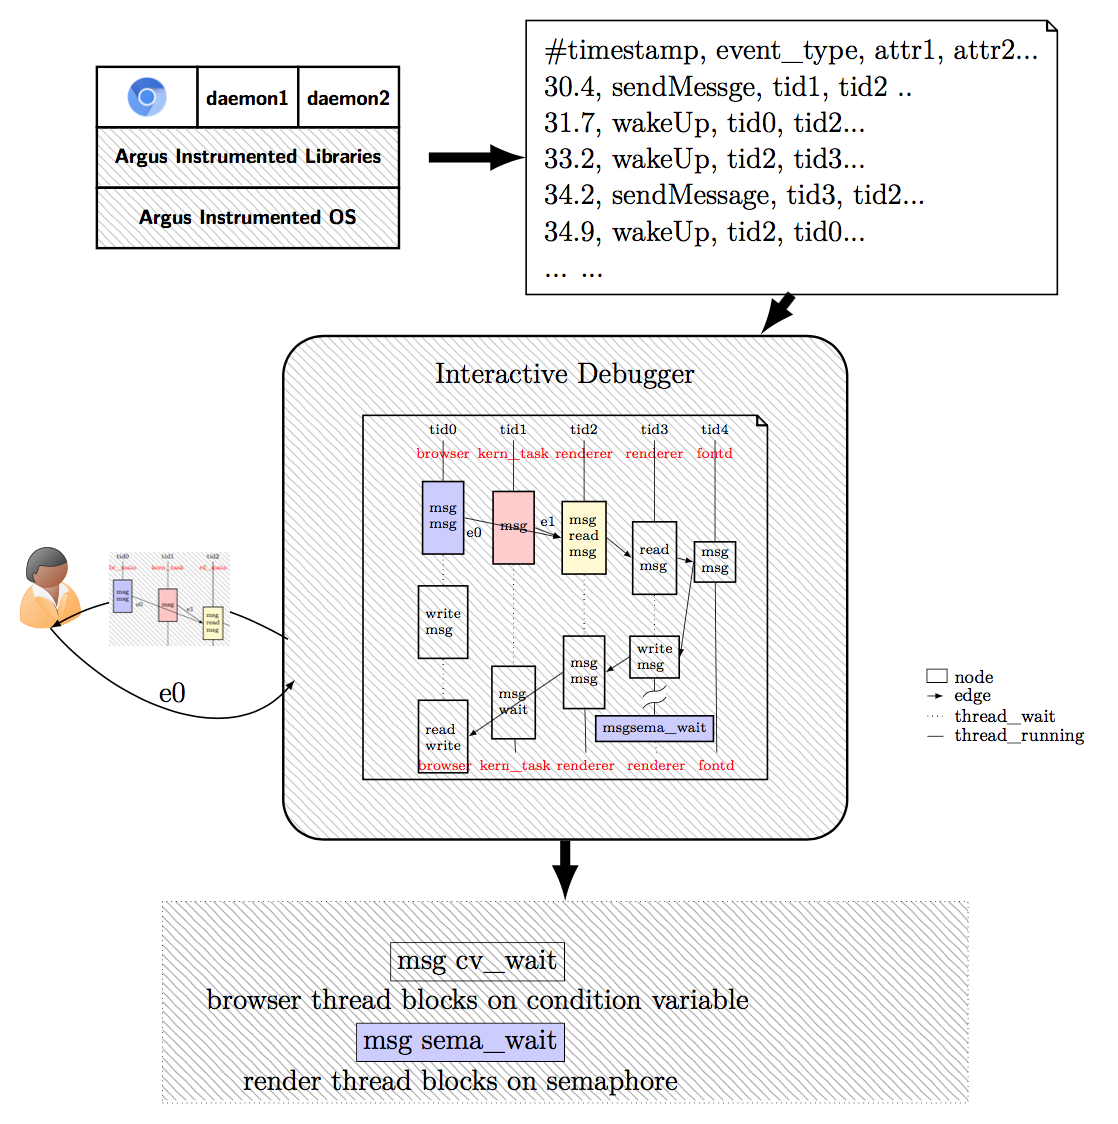
\includegraphics[width=\columnwidth]{figures/overview_tikz.png}
    \caption{\xxx Work Flow}
    \label{fig:argus-overview}
\end{figure}

In this section, we describe the steps a user takes to investigate a performance
anomaly with \xxx. Figure~\ref{fig:argus-overview} shows \xxx's work flow with
an example of a user investigating a performance problem in Chromium. The system
wide tracing tool, which collects data from \xxx instrumented library and
kernel, generates logs. They are transformed into an graph in \xxx's
graph construction component. 
Central to our system is our \emph{event graph}, a generalized control-flow
graph which includes inter-thread and inter-process dependencies.
%Diagnosis
%and inferences are performed within this graph, in a semi-automated fashion:
%\xxx performs searches to trace logical events as they
%flow through the system, and it judicially queries the user for guidance.
The generated graph is used by the interactive
debugger for causal path slicing and diagnosis. \xxx supports interactive
search, by providng information to the user and asking for decision, in case of
multiple predecessors in a vertex. As shown in Figure~\ref{fig:argus-overview},
the debugger asks user to choose one edge in a subgraph. After this step,
\xxx performs diagnosis algorithm and reports the root cause vertices. In the
example, the root cause is two vertices which form a circular wait acrossing
multiple threads.
%- sys-wide tracing => log
%- event graph
%- interacjjkjjktive search "find root cause"
%- root cause is two nodes, across multiple threads
%
%In this section, we describe the steps a user takes to investigate a performance
%anomaly with \xxx. Figure~\ref{fig:argus-overview} shows \xxx's work flow, which
%consists of two phases. A user runs command ``\vv{\xxx start}'' to enter the
%system-wide tracing phase, within which \xxx logs events as listed in Table
%~\ref{table:event_types} (\S\ref{subsec:eventgraph}). Whenever a user detects
%a performance issue such as a spinning cursor, she runs ``\vv{\xxx debug}'' to
%enter the diagnosis phase.
%
%%In the cases we consider, the flow of information across threads and processes
%%is essential to discovering the system state that leads to a performance bug.
%%\xxx recovers UI actions from logged data rather than being told the actions
%%that a user performs, because not all of them may be relevant to the true bug.
%%
%Central to our system is our \emph{event graph}, a generalized control-flow
%graph which includes inter-thread and inter-process dependencies. 
%Diagnosis
%and inferences are performed within this graph, in a semi-automated fashion:
%\xxx performs searches to trace logical events as they
%flow through the system, and it judicially queries the user for guidance.
% The event graph is described in further detail in \S\ref{subsec:eventgraph}.

Next, we describe how \xxx assists the user to diagnose a performance issue.

%fwd ref section on chromium, but first, how search event graph

\subsection{Diagnosis with Graph}\label{subsec:debug}

\begin{algorithm}[ht!]
    \caption{Diagnosis algorithm.}
    \label{alg:alg-diagnosis}
\begin{algorithmic}[1]
\Require{g - EventGraph; spinning\_node - the node in the UI thread when the spinning cursor occurs}
\Ensure{node\_vector - root cause node or the sliced path}
\Statex
\Function{Diagnose}{EventGraph g, Node *spinning\_node}
  \Switch {spinning\_node.block\_type}
    \Case {CPUBusy}
		\State {slice $\gets$ InteractiveSlice(spinning\_node)}
		\State\Return {slice}
	\EndCase
	\Case {Yield}
		\If {spinning\_node.NotContain(Share\_flag\_read\_Event)}
			\LineComment {Require users to annotate data flag}
			\State {abort()}
		\EndIf
		\LineComment {Fall through}
	\EndCase
	\Case {Wait}
		\LineComment {Find a baseline case where the wakeup occured}
		\State {normal\_nodes $\gets$ FindSimilar(spinning\_node)}
		\State {normal\_node $\gets$ Users.Pick(normal\_nodes)}
		\State {slice $\gets$ InteractiveSlice(normal\_node)} 	
		\State {$T_{spinning}$ $\gets$ spinning\_node.begin\_time}

		\For {$node$ $\gets$ $slice.begin().next()$ to $slice.end()$}
			\State {$T_{normal}$ $\gets$ node.end\_time}
			\State {$t$ $\gets$ node.thread}
			\State {$t\_nodes$ $\gets$ GetNodes(t, $T_{normal}$, $T_{spinning}$)}
			\For {$node_i$ $\gets$ $t\_nodes.begin()$ to $t\_nodes.end()$}
				\If {$node_i$.EventType == Wait}
					\State {node\_vector.append($node_i$)}
					\LineComment {Ask user if it is the root cause}
					\If {User.Yes}
						\State\Return {node\_vector}
					\Else
						\State {Diagnose($node_i$)}
					\EndIf
				\EndIf
			\EndFor
		\EndFor
		\LineComment {Fail to diagnose with blocking culprit, return the normal}
		\LineComment {node's parent for user to apply concrete debugging}
		\If {node\_vector.empty()}
			\State\Return {normal\_node.parent()}
		\EndIf
	\EndCase
  \EndSwitch
\EndFunction
\end{algorithmic}
\end{algorithm}


\begin{algorithm}[ht!]
    \caption{InteractiveSlicing algorithm.}
    \label{alg:alg-interactiveslicing}
\begin{algorithmic}[1]
\Require{g - EventGraph; node - the node user wants to slice from}
\Ensure{slice - causual path for node}
\Statex
\Function{InteractiveSlicing}{EventGraph g, Node *node}
\Loop
	\State{slice.append(node)}
	\If{node.parent().size() > 1}
		\State{node $\gets$ User.pick(candidates)}
		\If{node.NotExist()}
			\State\Return {slice}
		\EndIf
	\ElsIf{node.parent().size() == 1}
		\State{node $\gets$ node.parent().front()}
	\ElsIf{node.WeakEdges().size() > 0}
		\State{node $\gets$ User.Pick(weak edges)}
		\If{node.NotExist()}
			\State\Return {slice}
		\EndIf
	\Else
		\State\Return {slice}
	\EndIf
\EndLoop
\EndFunction
\end{algorithmic}
\end{algorithm}


Consider a common performance bug on macOS, the \emph{spinning cursor},
which indicates the current application's main thread has not processed
any UI events for over two seconds.  To initialize debugging a spinning
cursor, \xxx first constructs an event graph from the system-wide event
log recorded.  It then queries the event graph to find the ongoing event
in the application's main thread concurrent to the display of the spinning
cursor.  Given the event graph and the \spinningnode, \xxx runs
Algorithm~\ref{alg:alg-diagnosis} to interactively pinpoint the root
cause.

Specifically, upon examining what the main thread is actually doing, there
are three potential cases.

\begin{itemize}

	\item \textbf{LongRunning} (lines~\ref{a1:longrunning_begin}
		-~\ref{a1:longrunning_end}). The main thread is busy performing lengthy CPU
		operations. This case is the simplest, and \xxx traverses the event graph
		backwards to find a slice originating from the offending UI event to the
		long running CPU operations. This slice is particularly useful for further
		diagnosing the bug. As shown in FunctionXXX, \xxx may encounter vertices with
		multiple incoming edges or weak edges that may not reflect causality when
		traversing the graph. It queries the user to resolve them.

	\item \textbf{RepeatedYield} (lines~\ref{a1:repeatedyield_begin}
		-~\ref{a1:repeatedyield_end}). The main thread is in a yield loop, which
		is highly indicative it is waiting on a data flag (\eg, ``while(!done)
		thread\_switch();''). If \xxx cannot find any record of data flags in the
		\spinningnode, it terminates debugging by prompting the user to identify data
		flags and re-trace the application. Here we assume that the performance issue
		reproduces with a reasonable probability because, fortunately, a one-off issue
		that never reproduces is not as annoying as one that occurs frequently. If
		\xxx finds the data flag the \spinningnode is waiting for, it falls through to
		the next case.

	\item \textbf{LongWait} (lines~\ref{a1:longwait_begin}
		-~\ref{a1:longwait_end}). The main thread is in a lengthy blocking wait and
		the wake-up has been missing. \xxx handles this case by finding a baseline
		scenario where the wake-up indeed arrives, and then figures out which wake-up
		edge is missing in the spinning scenario along the expected wake-up path.
		Specifically, \xxx first finds a \similarnode to the spinning one based solely
		on the semantical events such as system calls in each vertex. It then traverses
		backwards from the \similarnode to find the baseline wake-up path. For each
		thread in the wake-up path, it examines the vertex in the thread right before
		the \spinningnode waits. If this vertex is also abnormal, \xxx appends it
		to the path of \rootcausenodes, and applies Function DiagnoseXX recursively
		diagnose ``the culprit of the culprit.'' For each such vertex, it queries the
		user to determine whether to proceed or stop because based on our experience
		the user needs to inspect only a few vertices to find the root cause.

\end{itemize}
%\vskip 0.1cm

Based on our results and experience, the first case is the most common, but the
second and third represent more severe bugs. Long-running CPU operations tend to
be more straightforward to diagnose with existing tools such as \spindump except
they do not connect CPU operations back to UI events. Repeated yielding or
long waiting cases involve multiple threads and processes, and are extremely
hard to understand and fix even for the application's original developers.
Therefore, issues remain unaddressed for years and significantly impact the
user experience. Algorithm~\ref{alg:alg-diagnosis} is semi-automated but can
integrate user input to leverage hypotheses or expert knowledge
as to why a hang may occur. Our results show that user inputs, albeit few, are
crucial in this process (\S\ref{sec:casestudy}).

\subsection{Chromium Spinning Cursor Example}

\begin{figure}[htb!]
    \centering
	%%\documentclass{article}
%%\usepackage{tikzpeople}
%%\usepackage{tikz}
%%\usetikzlibrary{shapes, shapes.misc}
%%\usetikzlibrary{arrows, arrows.meta, decorations.markings}
%%\usetikzlibrary{patterns}

%%\begin{document}
\begin{center}
\resizebox{\columnwidth}{!}{%
\begin{tikzpicture}[>=latex]
\tikzstyle{every node}=[font=\Large]
\tikzstyle{app} = [draw, very thick, minimum height=40em, minimum width=20em, fill=white, rectangle, font={\sffamily\bfseries}]
\tikzstyle{actionpoint} = [minimum width = 1em, fill = white]
\tikzstyle{point} = [thick, draw=red, cross out, inner sep = 0pt, minimum width = 0.5em, minimum height =0.5em]
%\tikzset{
%%ext/.pic={
%%\path [fill=white] (-0.2,0)to[bend left](0,0.1)to[bend right](0.2,0.2)to(0.2,0)to[bend left](0,-0.1)to[bend right](-0.2,-0.2)--cycle;
%%\draw (-0.2,0)to[bend left](0,0.1)to[bend right](0.2,0.2) (0.2,0)to[bend left](0,-0.1)to[bend right](-0.2,-0.2);
%%},
%point/.style={
%    thick,
%    draw=red,
%    cross out,
%    inner sep=0pt,
%    minimum width=4pt,
%    minimum height=4pt,
%}}

%draw applications
\node [app, name = browser]{};
\node (browsertag)[minimum width = 20em, above = -2em of browser] {Chromium Browser};
\node (browserend)[minimum width = 20em, below = 38em of browsertag] {};
\node (bt1begin)[minimum width = 8em, below left = 3em and -10em of browsertag]{main thread};
\node (bt1end)[minimum width = 8em, below left = 38em and -10em of browsertag]{};
\node (bt2begin)[minimum width = 8em, below right = 3em and -10em of browsertag]{worker thread};
\node (bt2end)[minimum width = 8em, below right = 38em and -10em of browsertag]{};
\draw [solid] (bt1begin) -- (bt1end);
\draw [solid] (bt2begin) -- (bt2end);
\node (1)[actionpoint, below of = bt1begin, node distance = 8em]{1};
\node (2)[actionpoint, below of = bt2begin, node distance = 9em]{2};
\node (9)[actionpoint, below of = 2, node distance = 16em] {9};
\node (10)[actionpoint, below of = 1, minimum width = 6em, minimum height = 2em, node distance = 18em, rotate=270]{timed wait};
%\node (11)[actionpoint, below of = 10, node distance = 4em]{};

\node [app, name = renderer, right of = browser, node distance = 25em]{};
\node (renderertag)[minimum width = 20em, above = -2em of renderer] {Chromium Renderer};
\node (rendererend)[minimum width = 20em, below = 38em of renderertag]{};
\node (bt3begin)[minimum width = 8em, below left = 3em and -10em of renderertag]{worker thread};
\node (bt3end)[minimum width = 8em, below left = 38em and -10em of renderertag]{};
\node (bt4begin)[minimum width = 8em, below right = 3em and -10em of renderertag]{main thread};
\node (bt4end)[minimum width = 8em, below right = 38em and -10em of renderertag]{};
\draw [solid] (bt3begin) -- (bt3end);
\draw [solid] (bt4begin) -- (bt4end);
\node (3)[actionpoint, below of = bt3begin, node distance = 10em]{3};
\node (4)[actionpoint, below of = bt4begin, node distance = 11em]{4};
\node (7)[actionpoint, below of = 4, node distance = 11em, rotate=270] {sema};
\node (8)[actionpoint, below of = 3, node distance = 13em]{8};

\node [app, name = fontd, right of = renderer, node distance = 25em]{};
\node (fontdtag)[minimum width = 20em, above = -2em of fontd] {fontd};
\node (fontdend)[minimum width = 20em, below = 38em of fontdtag]{};
\node (bt5begin)[minimum width = 20em, below = 3em of fontdtag]{worker thread};
\node (bt5end)[minimum width = 20em, below = 38em of fontdtag]{};
\draw [solid] (bt5begin) -- (bt5end);
\node (5)[actionpoint, below of = bt5begin, node distance = 14em] {5};
\node (6)[actionpoint, below of = 5, node distance = 3em] {6};

\draw [->] (1) -- (2);
\draw [->] (2) -- (3);
\draw [->] (3) -- (4);
\draw [->] (4) -- (5);
\coordinate[name = notarrive7, point, right of = 7, node distance = 1em];
\draw [->] (6) -- (notarrive7);
\coordinate[name = before7, above of = 7, node distance = 1em]{};
\draw [->] (before7) -- (8);
\draw [->] (8) -- (9);
\coordinate[name = notarrive10, point, right of = 10, node distance = 1em]{};
\draw [->] (9) -- (notarrive10);

\node (findfirstrect)[minimum width = 40em, minimum height = 4em, right of = 1, node distance = 13em, rotate = 355] {TextInputClientMsg\_FirstRectForCharacterRange};
\node (javascript)[minimum width = 4em, minimum height = 4em, above left = 0em and 2em of 7, rotate = 15] {Run\_Javascript};
\end{tikzpicture}
}
\end{center}
%%\end{document}

    \caption{Chromium Example}
    \label{fig:chromium-case-study}
\end{figure}
%   resolve symbol, save to log
%     search for set\_spinning
%     if found,
%       find main thread node at the time of set\_spinning
%     find fontd
%     manually check nodes in each thread immediately after the nodes in the slice (normal abnormal boundary)
%  output is a node, and a HTML dump of node and immediate predecessors and successors
% systems preference          
%  spinning node in UI thread is not waiting
%  so we look for messages, and find the diff

One of the authors experienced first-hand the aforementioned performance issue
in Chromium, an open-source browser engine that powers Google Chrome and,
starting recently, Microsoft Edge~\cite{chromiumurl}.  She tried to type in the
Chromium search box a Chinese word using SCIM, the default Chinese Input Method
Editor that ships with MacOS.  The browser appeared frozen and the spinning
cursor occurs for a few seconds.  Afterwards everything went back to normal.
This issue is reproducible and always ruins her experience, but it is quite
challenging to diagnose because two applications Chromium and SCIM and many
daemons ran and exchanged messages.  This issue was reported by other users for
other non-English input methods, too.

% issue, the user followed Figure 1.Figure~\ref{fig:argus-overview}
To diagnose this issue with \xxx, the author started system-wide tracing, and
then reproduced the spinning cursor with a Chinese search string typed via SCIM
while the page was loading. It produced normal cases for the very first few
characters, and the browser got blocked with the rest input as spinning cases.
The entire session took roughly five minutes.
%  spinning node
She then ran \xxx to construct the event graph. 
The graph was highly complex, with 
2,749,628 vertexes and 3,606,657 edges, almost fully connected. It spanned across 17 applications;
109 daemons including \vv{fontd}, \vv{mdworker}, \vv{nsurlsessiond} and
helper tools by applications; 126 processes; 679 threads, and 829,287
IPC messages. Given the scale of the graph and the diverse communication
patterns, it would be extremely challenging for prior automated causal tracing
tools~\cite{aguilera2003performance, zhang2013panappticon, attariyan2012x,
cohen2004correlating} because they handle a fairly limited set of patterns.
Tools that require manual schema~\cite{barham2004using, reynolds2006pip}, would
be prohibitive because developers would have to provide schema for all involved
applications and daemons.
% Perfect case for \xxx

% Figure 2....
Next she ran \xxx to find the \spinningnode in the main thread of the browser
process. \xxx returned a \vv{Wait} event on condition variable with timeout that
blocked the main thread for a few seconds. Thus \xxx compares the \spinningnode
to a similar one in normal case where the \vv{Wait} was signaled quickly. \xxx
reported three, and confirmed with the user which one she wanted.

\xxx then found the normal-case wake-up path which connects five threads, as is
shown in the example in Figure~\ref{fig:argus-overview}. The browser main thread
was signaled by a browser worker thread, which received IPC from a worker thread
of \vv{renderer} where the rendering view and WebKit code run. The worker thread
is woken up by the \vv{renderer} main thread, which in turn woken by fontd, the
font service daemon. \xxx further compared the wake-up path with the spinning
case, and returned the \vv{wait} event on semaphore in the \vv{renderer} main
thread, the culprit that delayed waking up the browser main thread over 4
seconds.

What caused the wait in the \vv{renderer} main thread though? She thus continued
diagnosis and recursively applied \xxx to the wait in \vv{renderer}, and got
the wake-up path. The culprit that delayed the semaphore was the timeouts in
the browser's main thread. At this point, a circular wait formed, as is shown
in Figure ~\ref{fig:chromium-case-study}. To understand what exactly happens in
the situation, she inspected the full call stacks by \xxx scripts, taking the
reported vertice from the renderer and the browser as input. Inspection reveals
that the \vv{renderer} requested the browser's help to render Javascript and
waited for reply with semaphore. The browser was waiting for the \vv{renderer}
to return the string bounding box and the \vv{renderer} was waiting for the
browser to help render Javascript. This circular wait was broken by a timeout in
the browser main thread (the \vv{wait} on cv timeout was 1,500 ms). While the
system was able to make progress, the next key press caused the spinning cursor
to display for another 1,500 ms. The timeout essentially converted a deadlock
into a livelock.

Finally, we verified our finding within chromium source code. Shortening the timeout interval
in the main browser thread proportionally shortens the waiting of the main
render thread on processing the javascript. Skipping certain javascripts
processing in the renderer thread cuts down the success rate of spinning case
reproducing.
% enough info for developer to fix issue once and for all

\subsection{Limitations}
\xxx is designed to support interactive debugging of performance
issues. It sometimes requires the user to reproduce a performance issue so
\xxx can capture more fine-grained event traces such as accesses to data
flags.  Fortunately, a performance issue that almost never reproduces is
probably not as annoying as one that occurs frequently.

We implemented \xxx in the closed-source macOS which presents a harsh test
for \xxx, but we have not ported \xxx to other operating systems yet. It is
possible that the ideas and techniques do not generalize to other operating
systems. However, modern operating systems share many similarities, and inspire each others' designs,
so we are hopeful that the ideas in \xxx are
generally applicable. Similarly, the applications and performance issues used in
our evaluation may be non-representative, though we strive to cover a
diverse set of common applications ranging from browsers to text editors.
